\documentclass[crop,tikz]{standalone}

\providecommand{\rootdir}{..}
\usetikzlibrary{calc, positioning, shapes.geometric}
\tikzstyle{arrow} = [thick,->,>=stealth]

% The Tableau20 colours
\definecolor{TabLightOrange}{RGB}{255,187,120}
\definecolor{TabOrange}{RGB}{255,127,14}
\definecolor{TabLightBlue}{RGB}{174,199,232}
\definecolor{TabBlue}{RGB}{31,119,180}
\definecolor{TabGreen}{RGB}{44,160,44}
\definecolor{TabLightGreen}{RGB}{152,223,138}
\definecolor{TabSalmon}{RGB}{255,152,150}
\definecolor{TabRed}{RGB}{214,39,40}
\definecolor{TabPurple}{RGB}{148,103,189}
\definecolor{TabLightPurple}{RGB}{197,176,213}
\definecolor{TabLightPink}{RGB}{247,182,210}
\definecolor{TabPink}{RGB}{227,119,194}
\definecolor{TabLightBrown}{RGB}{196,156,148}
\definecolor{TabBrown}{RGB}{140,86,75}
\definecolor{TabGray}{RGB}{127,127,127}
\definecolor{TabOlive}{RGB}{188,189,34}
\definecolor{TabLightOlive}{RGB}{219,219,141}
\definecolor{TabLightGray}{RGB}{199,199,199}
\definecolor{LightCyan}{RGB}{158,218,229}
\definecolor{TabCyan}{RGB}{23,190,207}

\begin{document}
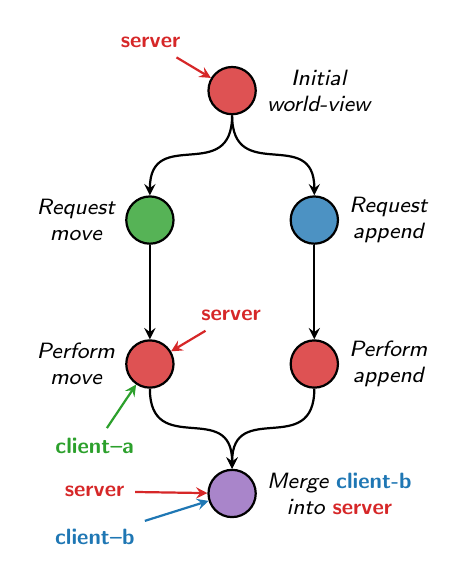
\begin{tikzpicture}
  [ every node/.style={font=\footnotesize\sffamily}
  , every label/.style={align=center}
  , c/.style = {
    , circle
    , prefix after command= {\pgfextra{\tikzset{
          every label/.style={align=center, font=\footnotesize\itshape\sffamily}
        }}}
    , minimum size = 0.6cm
    , inner sep = 0pt
    , draw = black
  }
  , inner-c/.style = {
    , minimum size = 0.35cm
    , draw
    , circle
    , inner sep = 0pt
  }
  , server/.style = {fill=TabRed!80}
  , merge/.style = {fill=TabPurple!80}
  , client-a/.style = {fill=TabGreen!80}
  , client-b/.style = {fill=TabBlue!80}
  , arrow={thick, ->, >=stealth}
  , node distance = 1.2cm and 0.6cm
  ]
  \def\controlsep{1.2}


  \onslide<2->{
    \node[c, server, label=right:{Initial\\world-view}] (s1) {};
  }

  \onslide<2-6>{
    \node[color=TabRed, above left = 2mm and 0.3cm of s1] (server-label) {\textbf{server}};
    \draw[TabRed, ->] (server-label) -- (s1);
  }
  
  \onslide<3->{
    \node[c, client-a, below left = of s1, label=left:{Request\\move}] (a) {};
    \draw[->] (s1) .. controls +(0,-\controlsep) and +(0,\controlsep) .. (a);
  }

  \onslide<5->{
    \node[c, client-b, below right = of s1, label=right:{Request\\append}] (b) {};
    \draw[->] (s1) .. controls +(0,-\controlsep) and +(0,\controlsep) .. (b);
  }
  
  \onslide<7->{
    \node[c, server, below = of a, label=left:{Perform\\move}] (sa) {};
    \draw[->] (a) -- (sa);
  }

  \onslide<7-9>{
    \node[color=TabRed, above right = 2mm and 0.3cm of sa] (server-label) {\textbf{server}};
    \draw[TabRed, ->] (server-label) -- (sa);
  }

  \onslide<8->{
    \node[color=TabGreen, below = 0.5cm of sa, xshift=-0.7cm] (clienta-label) {\textbf{client--a}};
    \draw[TabGreen, ->] (clienta-label) -- (sa);
  }
  
  \onslide<9->{
    \node[c, server, below = of b, label=right:{Perform\\append}] (sb) {};
    \draw[->] (b) -- (sb);
  }

  \onslide<10->{
    \node[c, merge, below right = of sa, label=right:{Merge \textcolor{TabBlue}{\textbf{client-b}}\\into \textcolor{TabRed}{\textbf{server}}}] (merge) {};
    \draw[->] (sa) .. controls +(0,-\controlsep) and +(0,\controlsep) .. (merge);
    \draw[->] (sb) .. controls +(0,-\controlsep) and +(0,\controlsep) .. (merge);

    \node[color=TabRed, below = 0.15cm of clienta-label] (server-label) {\textbf{server}};
    \draw[TabRed, ->] (server-label) -- (merge);
  }
  
  \onslide<11->{
    \node[color=TabBlue, below = 0.15cm of server-label] (clientb-label) {\textbf{client--b}};
    \draw[TabBlue, ->] (clientb-label) -- (merge);
  }
\end{tikzpicture}
\end{document}